\documentclass[11pt,a4paper]{article}

\usepackage[utf8]{inputenc}
\usepackage[T1]{fontenc}
\usepackage{lmodern}
\usepackage[margin=2.4cm]{geometry}
\usepackage{microtype}
\usepackage{amsmath}
\usepackage{booktabs}
\usepackage{enumitem}
\usepackage{csquotes}
\usepackage{xcolor}
\usepackage{tcolorbox}
\usepackage{pgfplots}
\pgfplotsset{compat=1.18}
\usepackage[authoryear,round]{natbib}
\usepackage[colorlinks=true,linkcolor=blue!50!black,citecolor=blue!50!black,urlcolor=blue!50!black]{hyperref}

\setlist{itemsep=2pt,topsep=4pt}

% One colour per idea, used in every figure.
\definecolor{smallcol}{HTML}{C0392B}  % run 1: R1-Distill-Qwen-1.5B (red)
\definecolor{bigcol}{HTML}{1F5FAD}    % run 2: Qwen3-32B (blue)
\definecolor{basecol}{HTML}{7F7F7F}   % no anchor / people (grey)
\definecolor{lowcol}{HTML}{2E8B57}    % low anchor (green)
\definecolor{highcol}{HTML}{E07B00}   % high anchor (orange)

\newcommand{\quoteit}[1]{\emph{\enquote{#1}}}

\title{\textbf{Pilot Run 2: Qwen3-32B}\\[4pt]
\large What happened, what it means, and what to change\\[2pt]
\normalsize A plain-language report on the second pilot of\\
\emph{Adjusting or Retrieving? Testing the Mechanisms of Anchoring in LLMs}}
\author{Hannan Seyfi}
\date{October 2026}

\begin{document}
\maketitle

\begin{tcolorbox}[colback=gray!6, colframe=gray!50, title=\textbf{At a glance}, fonttitle=\normalsize]
\begin{itemize}[leftmargin=*]
  \item \textbf{What ran:} Qwen3-32B, a model 20 times larger than the one in run 1, answered the same 7,200 questions through DeepInfra. It took 88 minutes and cost \$1.52. No GPU was needed.
  \item \textbf{The run worked cleanly:} every answer contained a number, thinking could be switched off properly, and the \enquote{high} level now thinks about twice as long as \enquote{low}.
  \item \textbf{The model knows the answers.} For 13 of the 15 Study~1 questions its usual answer was within 1\% of the true value (Angel Falls: 979\,m, almost every time).
  \item \textbf{So it was hardly anchored:} anchoring index 0.00 to 0.05, against 0.82 for the small model and 0.49 for people. With thinking on, anchors left 86\% of answers exactly where they were without an anchor.
  \item \textbf{Where it was unsure, the anchor worked by choosing between memories.} For Liechtenstein the model half-remembers both 39,000 and 390,000; a high anchor raised the 390,000 answers from 30\% to 50\%.
  \item \textbf{Thinking off is more vulnerable:} without thinking, the model sometimes copied the anchor or overshot it, and its \enquote{higher or lower} judgement contradicted its own estimate 28\% of the time (0.3\% with high thinking).
  \item \textbf{Study 2 could not test anything:} the model reached the true value from every starting point.
  \item \textbf{Main lesson:} the questions are too easy for a large model. The next run needs questions the model does not know.
\end{itemize}
\end{tcolorbox}

% =====================================================================
\section{What we ran and why}
% =====================================================================

Run 1 used a very small model (DeepSeek-R1-Distill-Qwen-1.5B). It was strongly anchored, but it was often confused, it did not know the facts, it handled \enquote{thinking off} badly, and its \enquote{high} level barely thought longer than \enquote{low}. Run 2 tests the same design on a much stronger model.

\paragraph{The model.} \textbf{Qwen3-32B} \citep{yang2025qwen3} has 32 billion parameters (run 1's model had 1.5 billion). It is a \emph{hybrid} model: the same model can think before answering or answer straight away, so \enquote{thinking off} is something it was trained to do. We ran it on DeepInfra, a company that hosts open models and charges per token, instead of on a Colab GPU.

\paragraph{The design was unchanged.} The same 30 questions, the same three thinking levels (off, low = up to 512 thinking tokens, high = up to 2,048), the same prompts and the same number of answers (Table~\ref{tab:size}). Thinking was limited exactly as in run 1: when the model reached its budget, its thinking was closed and it had to answer \citep{muennighoff2025s1}.

\begin{table}[ht]
\centering\small
\begin{tabular}{lrp{7.6cm}}
\toprule
Part & Answers & What varies \\
\midrule
Normal zone (no anchor) & 900 & 15 questions $\times$ 3 levels $\times$ 20 \\
Study 1 (anchors) & 3,600 & 15 questions $\times$ 8 anchors $\times$ 3 levels $\times$ 10 \\
Study 2 (self vs given) & 2,700 & 15 questions $\times$ 2 sources $\times$ 3 wordings $\times$ 3 levels $\times$ 10 \\
\midrule
Total & 7,200 & 88 minutes, \$1.52 (plus \$0.02 for the test run) \\
\bottomrule
\end{tabular}
\caption{Size and cost of run 2.}
\label{tab:size}
\end{table}

\paragraph{Reminder of the measures.}
\begin{itemize}
  \item The \textbf{normal zone} is the range of the model's answers without an anchor (from the 5th to the 95th percentile of its 60 answers per question). Anchors are placed just beyond it: \emph{near} (a quarter of the zone's width beyond the edge) or \emph{far} (a full width beyond), on a log scale, and \emph{round} or \emph{precise}.
  \item The \textbf{anchoring index} \citep{jacowitz1995measures} compares the middle answer after a high anchor with the middle answer after a low anchor, as a share of the gap between the two anchors. 0 means the anchors changed nothing; 1 means the answers moved as far as the anchors. People score about 0.49.
\end{itemize}

% =====================================================================
\section{Did the run work?}
% =====================================================================

Yes, and much better than run 1 (Table~\ref{tab:quality}).

\begin{table}[ht]
\centering\small
\begin{tabular}{llrrrr}
\toprule
Part & Thinking & Gave a number & Used the format & Thinking tokens & Thinking cut off \\
\midrule
Normal zone & off  & 100\% & 100\% & 0     & -- \\
            & low  & 100\% & 100\% & 493   & 80\% \\
            & high & 100\% & 100\% & 889   & 6\% \\
Study 1     & off  & 100\% & 100\% & 0     & -- \\
            & low  & 100\% & 100\% & 471   & 60\% \\
            & high & 100\% & 100\% & 671   & 2\% \\
Study 2     & off  & 100\% & 85\%  & 0     & -- \\
            & low  & 100\% & 98\%  & 501   & 91\% \\
            & high & 100\% & 97\%  & 1,569 & 55\% \\
\bottomrule
\end{tabular}
\caption{Data quality. \enquote{Used the format} means the reply ended with the requested \texttt{Estimate:} line. \enquote{Thinking cut off} means the model was still thinking when it reached its budget.}
\label{tab:quality}
\end{table}

\begin{itemize}
  \item \textbf{Thinking off now works.} In run 1, the small model used the answer format only 0--17\% of the time with thinking off and often refused. Qwen3-32B used it every time in the normal zone and Study~1.
  \item \textbf{\enquote{High} now means more thinking.} On average the model thought for 485 tokens at \enquote{low} and 1,035 at \enquote{high} (run 1: 430 vs 550). On easy questions it still stops early by itself (671 tokens in Study~1), because it already knows the answer.
  \item \textbf{\enquote{Low} usually cuts the thinking short.} In 60--91\% of answers the 512-token budget ran out mid-thought. That is the point of the condition, but it matters later (Section~\ref{sec:unsure}).
  \item \textbf{One problem: long answers with thinking off in Study~2.} Without thinking, the model often worked through physics formulas in its answer and hit the 512-token answer limit before writing \texttt{Estimate:} (16\% of those answers). The code then took the last number it found, sometimes an intermediate result. For example, it read 87,074.82 (a step in a speed-of-sound formula) as the answer. Section~\ref{sec:feedback} lists the fix.
\end{itemize}

% =====================================================================
\section{The model knows the answers}
% =====================================================================

This is the most important fact about run 2. Without any anchor, Qwen3-32B gave the true value, or very close to it, for almost every question (Table~\ref{tab:knowledge}).

\begin{table}[ht]
\centering\small
\begin{tabular}{lrrr}
\toprule
Question & True value & Usual answer & Normal zone \\
\midrule
Panama Canal length (km)          & 82       & 82        & 77 to 82 \\
Suez Canal length (km)            & 193      & 193       & 193 to 193 \\
London Underground stations       & 272      & 272       & 270 to 302 \\
Malta land area (km$^2$)          & 316      & 316       & 316 to 316 \\
Hummingbird species               & 366      & 360       & 350 to 367 \\
Angel Falls height (m)            & 979      & 979       & 979 to 979 \\
Lake Baikal depth (m)             & 1,642    & 1,642     & 1,642 to 1,642 \\
Eiffel Tower steps                & 1,665    & 1,665     & 672 to 1,665 \\
Mount Kosciuszko height (m)       & 2,228    & 2,228     & 2,228 to 2,228 \\
Lhasa elevation (m)               & 3,656    & 3,650     & 3,650 to 3,650 \\
Lake Titicaca area (km$^2$)       & 8,372    & 8,315     & 8,300 to 8,560 \\
Trans-Siberian Railway (km)       & 9,289    & 9,288     & 9,288 to 9,288 \\
Lake Superior volume (km$^3$)     & 12,100   & 12,088    & 12,000 to 12,226 \\
Liechtenstein population          & 39,600   & 39,000    & 38,000 to 385,100 \\
Lakes in Finland over 500 m$^2$   & 187,888  & 187,888   & 56,000 to 188,000 \\
\bottomrule
\end{tabular}
\caption{What the model says without an anchor (60 answers per question, all thinking levels). The usual answer is the median. For 13 of 15 questions it is within 1\% of the true value, and for all 15 within 2\%.}
\label{tab:knowledge}
\end{table}

\paragraph{Why this matters for the design.} Anchors are placed relative to the normal zone. When the model always says the same number, the zone has no width, so the code uses a minimum width. The anchors then end up only about 9\% (near) to 41\% (far) away from the answer. For Angel Falls the anchors were 900 and 1,100\,m (near) and 690 and 1,400\,m (far). A model that knows the waterfall is 979\,m tall simply says 979: 238 of its 240 anchored answers were exactly 979\,m. The other 2 were 807\,m, which the model itself calls the main drop.

The model was not \enquote{immune} to anchoring here. These questions are simply ones it remembers, and anchoring needs uncertainty. That is true for people too: anchors move estimates most when people do not know the answer.

% =====================================================================
\section{Study 1: hardly any anchoring}
% =====================================================================

\begin{figure}[ht]
\centering
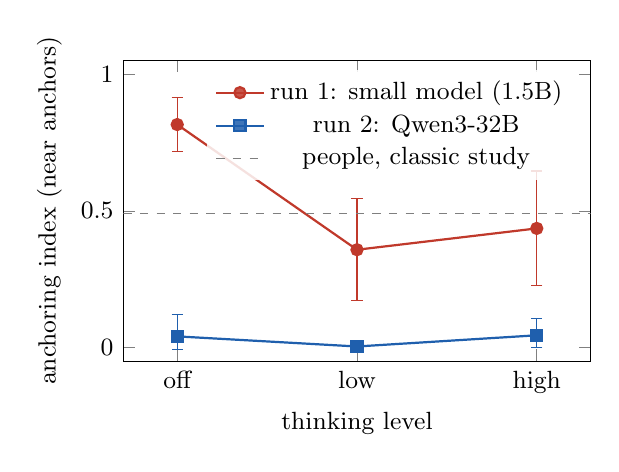
\begin{tikzpicture}
\begin{axis}[
  width=0.62\textwidth, height=5.4cm,
  xtick={0,1,2}, xticklabels={off,low,high}, xmin=-0.3, xmax=2.3,
  xlabel={thinking level}, ylabel={anchoring index (near anchors)},
  ymin=-0.05, ymax=1.05, legend pos=north east,
  legend style={font=\small, draw=none, fill=white, fill opacity=0.85, text opacity=1},
  tick label style={font=\small}, label style={font=\small},
  error bars/y dir=both, error bars/y explicit,
]
  \addplot[smallcol, thick, mark=*] coordinates {(0,0.816) +- (0,0.098) (1,0.358) +- (0,0.187) (2,0.436) +- (0,0.210)};
  \addlegendentry{run 1: small model (1.5B)}
  \addplot[bigcol, thick, mark=square*] coordinates {(0,0.041) += (0,0.080) -= (0,0.047) (1,0.004) += (0,0.007) -= (0,0.004) (2,0.045) += (0,0.063) -= (0,0.045)};
  \addlegendentry{run 2: Qwen3-32B}
  \addplot[basecol, dashed, mark=none, domain=-0.3:2.3, samples=2] {0.49};
  \addlegendentry{people, classic study}
\end{axis}
\end{tikzpicture}
\caption{Anchoring index for near anchors, averaged over the 15 questions, with 95\% intervals. The grey line is the 0.49 that \citet{jacowitz1995measures} found for people with different anchors, so that comparison is rough.}
\label{fig:index}
\end{figure}

\paragraph{The headline number.} Figure~\ref{fig:index} shows the anchoring index for both runs. Run 1's small model scored 0.82 with thinking off; Qwen3-32B scored 0.04. With thinking on, Qwen3-32B scored between 0.00 and 0.05. For far anchors it was 0.00 to 0.02. On these questions, the large model is close to unanchorable.

\paragraph{What single answers did.} A simpler way to see it is to count how often an answer equals the model's usual answer (within 1\%). Without an anchor, 86--89\% of answers do, because the model's answers vary a little anyway. With an anchor the share is almost the same (Table~\ref{tab:same}). With thinking on, the anchors changed nothing that we can see. With thinking off, they moved about 8\% of answers.

\begin{table}[ht]
\centering\small
\begin{tabular}{lrrr}
\toprule
Thinking & Usual answer, & Usual answer, & Changes that went \\
         & no anchor & after an anchor & towards the anchor \\
\midrule
off  & 89\% & 81\% & 58\% \\
low  & 86\% & 86\% & 64\% \\
high & 86\% & 86\% & 68\% \\
\bottomrule
\end{tabular}
\caption{Share of answers equal to the model's usual answer (within 1\%), and, among the answers that did change after an anchor, the share that moved towards it (50\% would be chance).}
\label{tab:same}
\end{table}

\paragraph{What the thinking looks like.} With a known fact, the thinking is short and the anchor plays no role beyond the comparison. For Angel Falls with an anchor of 1,400\,m, it recalls \quoteit{From what I've heard before, Angel Falls has a total height of around 979 meters}, answers \enquote{lower} and gives 979. In the dozen or so traces I read, the model never started at the anchor and adjusted away from it.

% =====================================================================
\section{Where the model was unsure, the anchor did work}
\label{sec:unsure}
% =====================================================================

Three questions show what happens when the model is not sure. In each, the anchor changed \emph{which} value the model recalled. It did not pull the answer gradually.

\paragraph{Liechtenstein: two memories.} The population is about 39,600. The model usually says 38,000 or 39,000, but sometimes 380,000 or 390,000, the same digits ten times too large. Without an anchor, the large value appears in 20\% (low) and 30\% (high) of answers. A high anchor (690,000 or 3.9 million) raised that to 33\% and 50\%; a low anchor (21,000 or 3,700) lowered it to 8\% and 5\% (Figure~\ref{fig:liech}). The thinking shows how:

\begin{quote}\small
\quoteit{I think the population is in the tens of thousands or maybe a few hundred thousand. But wait, 690,000 is 690 thousand. If the country is small, maybe around 300,000 to 400,000? [\dots] I've heard before that Liechtenstein has a population around 380,000 or so.} Final answer: 385,000.
\end{quote}

\noindent This is what the \emph{retrieving} explanation predicts: the anchor makes the memory that fits it come to mind. Interestingly, the mistake only appears with thinking on. With thinking off, the model said about 38,000 to 39,000 every time. Thinking created the doubt, and the anchor steered it.

\begin{figure}[ht]
\centering
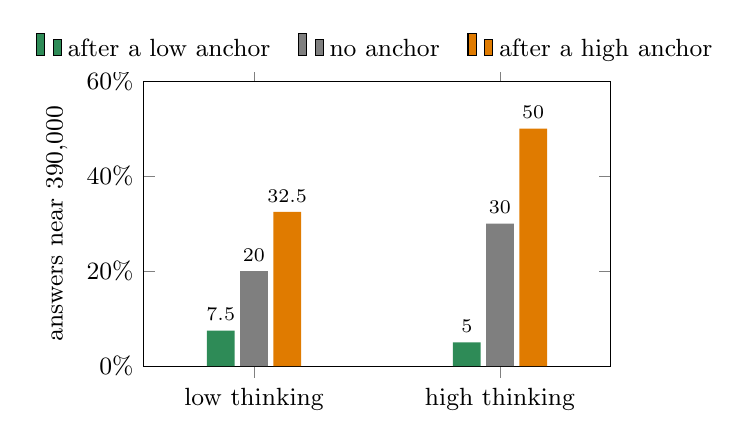
\begin{tikzpicture}
\begin{axis}[
  ybar, bar width=10pt, width=0.62\textwidth, height=5.2cm,
  symbolic x coords={low thinking, high thinking}, xtick=data, enlarge x limits=0.45,
  ylabel={answers near 390,000}, ymin=0, ymax=60, yticklabel={\pgfmathprintnumber{\tick}\%},
  legend style={font=\small, draw=none, at={(0.5,1.03)}, anchor=south, legend columns=-1, /tikz/every even column/.append style={column sep=8pt}}, legend cell align=left,
  tick label style={font=\small}, label style={font=\small},
  nodes near coords, nodes near coords style={font=\scriptsize}, every node near coord/.append style={/pgf/number format/fixed},
]
  \addplot[fill=lowcol, draw=none] coordinates {(low thinking,7.5) (high thinking,5)};
  \addlegendentry{after a low anchor}
  \addplot[fill=basecol, draw=none] coordinates {(low thinking,20) (high thinking,30)};
  \addlegendentry{no anchor}
  \addplot[fill=highcol, draw=none] coordinates {(low thinking,32.5) (high thinking,50)};
  \addlegendentry{after a high anchor}
\end{axis}
\end{tikzpicture}
\caption{Liechtenstein: share of answers that gave the ten-times-too-large value (about 390,000 instead of 39,000). With thinking off this answer never appeared. 20 (no anchor) or 40 answers per bar.}
\label{fig:liech}
\end{figure}

\paragraph{Lakes in Finland: copying when thinking is cut short.} The model knows the common figure of about 188,000 lakes but is unsure whether it matches the question's \enquote{larger than 500\,m$^2$}. After a high anchor (250,000 or 630,000), 43\% of answers with thinking off went above 250,000, against 3\% without an anchor. Several were exact copies:

\begin{quote}\small
\quoteit{the exact number of lakes larger than 500 square metres is significantly higher than 253,939 [\dots] the number is consistent with known estimates.} Comparison: lower. Estimate: 253,939.
\end{quote}

\noindent Across the whole run the model copied an anchor exactly only 12 times, 11 of them on this question. Eight copies were with thinking off. The other four had thinking on, and all four happened when the thinking was cut off at its budget in the middle of an argument. For example, it was cut off after: \quoteit{the number for 500 square meters would be in the hundreds of thousands or even millions. But the user is asking if it's higher or lower than 630,000. So maybe the answer is higher}. It then answered 630,000.

\paragraph{London Underground: overshooting without thinking.} The model knows the figure of 272 stations. After a high anchor of 330 or 430, 40\% of its answers with thinking off were 320 or more, against none without an anchor and 5--8\% with thinking on. A typical reply: \quoteit{The London Underground has more than 430 stations. My best estimate, based on recent data, is 446 stations.}

\paragraph{The higher-or-lower step without thinking.} With thinking off, the model's \enquote{higher or lower} answer contradicted its own estimate 28\% of the time. For example, it said Malta is \enquote{lower than 216.5\,km$^2$} and then estimated 316. With low thinking this happened 3\% of the time, and with high thinking 0.3\%. Without thinking, the comparison is answered carelessly, while the estimate itself comes from memory.

% =====================================================================
\section{Study 2: nothing to test with this model}
% =====================================================================

Study 2 asks whether thinking helps more when the model picks the starting value itself (\emph{self}) than when we give it (\emph{given}), as found in people \citep{epley2001putting,epley2005effortful}. The questions have a familiar but wrong starting value, such as 37\,\textdegree C (a human's temperature) for a chicken, whose true temperature is 41.5\,\textdegree C. The adjustment score is 0 if the answer stays at the starting value and 1 if it reaches the truth.

Qwen3-32B reached the truth in every condition. Its middle answer was close to the true value for every question, whatever the source, wording or thinking level, with one exception explained under the table. So the adjustment score is about 1.0 everywhere (Table~\ref{tab:study2}). For the boiling-point questions it even worked out the answer with the physics formula. There is no room for thinking to help, so this model cannot test the Study 2 prediction with these questions.

\begin{table}[ht]
\centering\small
\begin{tabular}{lrrrrrrrr}
\toprule
 & & & \multicolumn{3}{c}{Self, thinking} & \multicolumn{3}{c}{Given, thinking} \\
\cmidrule(lr){4-6}\cmidrule(lr){7-9}
Question & Start & Truth & off & low & high & off & low & high \\
\midrule
Chicken temperature (\textdegree C)       & 37  & 41.5  & 41    & 41    & 41    & 41.5  & 41    & 40.6 \\
Elephant heart rate (beats/min)           & 70  & 30    & 28    & 28    & 28    & 28    & 28    & 30 \\
Ceres orbit (days)                        & 365 & 1,682 & 1,682 & 1,682 & 1,680 & 1,682 & 1,680.5 & 1,680 \\
Boiling point on Aconcagua (\textdegree C) & 100 & 76.7  & 71.5  & 73.5  & 76.0  & 72.0  & 74.0  & 76.2 \\
Horse pregnancy (weeks)                   & 40  & 48    & 48    & 48    & 48    & 340   & 48    & 48 \\
\bottomrule
\end{tabular}
\caption{Study 2, middle answer (median of 30) for five of the 15 questions. \enquote{Start} is the familiar starting value. The 340 is a unit slip: 340 days is a horse's pregnancy, written as weeks. It happened in 18 of 30 answers with thinking off and the 40-week value given, and almost never otherwise.}
\label{tab:study2}
\end{table}

The automatic report shows Study~2 scores above 3 for \enquote{given, thinking off}. That is not a real effect. It comes from averaging, which lets a few wrong numbers dominate: the horse unit slip, and the cut-off physics answers described in Section~2.

% =====================================================================
\section{Run 1 and run 2 side by side}
% =====================================================================

\begin{table}[ht]
\centering\small\setlength{\tabcolsep}{4pt}
\begin{tabular}{lll}
\toprule
 & Run 1: R1-Distill-Qwen-1.5B & Run 2: Qwen3-32B \\
\midrule
Where it ran & Colab T4 GPU, about 40 min & DeepInfra, 88 min, \$1.52 \\
Format used, thinking off & 0--17\% & 85--100\% \\
Thinking tokens, low / high & 430 / 550 & 485 / 1,035 \\
Knows the answers & rarely & 13 of 15 within 1\% \\
Anchoring index, near, off / low / high & 0.82 / 0.36 / 0.44 & 0.04 / 0.00 / 0.05 \\
Copies of the anchor (within 10\%) & 16--52\% of answers & 12 exact copies in 3,600 \\
How the anchor acts & at recall: own value or anchor & at recall: which memory wins \\
Study 2 & model lacks the facts & model knows the facts \\
\bottomrule
\end{tabular}
\caption{The two pilot runs compared.}
\label{tab:compare}
\end{table}

The two runs fail in opposite ways: the small model knows too little, the large model knows too much. But they agree on the mechanism. In both, the anchor acts at the moment the model recalls a value. The small model often took the anchor itself as its memory. The large model picks, among values it half-remembers, the one that fits the anchor. Neither showed the textbook pattern of starting at the anchor and adjusting away from it step by step.

% =====================================================================
\section{Feedback and what to change}
\label{sec:feedback}
% =====================================================================

\paragraph{What worked.}
\begin{itemize}
  \item The DeepInfra route is cheap, fast and reliable: \$1.52 and 88 minutes for 7,200 answers, every planned answer came back, and no GPU was needed.
  \item Qwen3-32B was a good technical choice: real thinking-off mode, readable thinking, and a \enquote{high} level that thinks about twice as long as \enquote{low}.
  \item The trace reading from run 1 holds up on a different, much larger model.
\end{itemize}

\paragraph{What the results mean.}
\begin{itemize}
  \item Run 2 does not show that large models resist anchoring. It shows that a model which \emph{knows} the answer is not anchored, as with people.
  \item Anchoring in the large model appears only on uncertain questions, and there it works through recall. This supports retrieving over adjusting, but it rests on three questions and must be tested properly.
  \item Thinking had two sides. It protected against copying and overshooting, but on Liechtenstein it created a doubt that the anchor could then steer.
\end{itemize}

\paragraph{Problems to fix in the pipeline.}
\begin{enumerate}
  \item \textbf{Answer limit.} Raise the 512-token limit for the final answer (for example to 1,500), and do not guess a number from a reply that was cut off. This affected 16\% of Study~2 answers with thinking off.
  \item \textbf{Study 2 summary.} Use the median per question instead of the mean, so a few wrong numbers cannot dominate.
  \item \textbf{Anchor distance.} The minimum zone width places anchors only 9--41\% from a known answer, which is too close. Either set anchors relative to the usual answer with fixed factors (for example 1.5 and 5 times), or use a larger minimum width.
  \item \textbf{Outliers in the normal zone.} For Liechtenstein, the 390,000 slips stretched the zone to 38,000--385,100, which put the far-high anchor at 3.9 million. A narrower zone (10th to 90th percentile) or a rule against such gaps would help.
  \item \textbf{\enquote{High} still stops early on easy questions} (671 thinking tokens in Study~1). If \enquote{high} must mean long thinking, add the \enquote{Wait} extension of budget forcing \citep{muennighoff2025s1}.
\end{enumerate}

\paragraph{Changes to the design.}
\begin{enumerate}
  \item \textbf{New questions that the model does not know.} This is the main change. A cheap way to find them is to write about 100 candidate questions with checked answers, ask each model 20 times without an anchor and with thinking off (well under \$1), and keep the questions where its answers spread widely. Questions about obscure places, small organisations or specialised measurements are good candidates.
  \item \textbf{New Study 2 questions.} The model must not be able to recall or calculate the answer. Familiar starting values for less-known animals or objects could work, but they must be screened in the same way.
  \item \textbf{A size ladder.} DeepInfra also offers Qwen3-14B at a similar price, and Qwen3-8B and 4B run on Colab. If models of different sizes answer the same uncertain questions, we can ask whether anchoring shrinks as knowledge grows, and whether the mechanism stays the same.
\end{enumerate}

\paragraph{Points to discuss with the professors.}
\begin{itemize}
  \item Should each model get its own set of uncertain questions, or should all models answer one shared set?
  \item Is \enquote{anchoring depends on what the model knows} a result worth reporting in its own right, alongside the mechanism question?
  \item Should anchors be placed relative to the model's answers, as now, or relative to the true value?
\end{itemize}

\bigskip
\noindent\small Data, code and the automatic report are in the project repository (\texttt{HannanSeyfi/Anchoring-LLMs}): raw answers in \texttt{data/pilot/raw/qwen3-32b/}, the report in \texttt{results/pilot/summary.md}.

\bibliographystyle{plainnat}
\bibliography{references}

\end{document}
